En este capítulo se detalla cada uno de los puntos llevados a cabo para la realización de este proyecto, empezando por definir la propuesta realizada, luego explicar el proceso ingenieril llevado a cabo y terminar desglosando el trazado de la ejecución de este proyecto.

\section{Propuesta}

El trabajo propuesto tiene como objetivo la creación de un elemento software funcional que, usando el paradigma lógico explicado en la Sección \ref{subsec:asp}, permita la generación de un área que contenga una planificación de un polígono industrial que pueda ser generado y jugado dentro del mapa de \cities. Así mismo incluirá una interfaz gráfica interactuable que permitan al usuario marcar que zonas del terreno deben generarse y cuales no, indicando su contenido antes de lanzar el proceso de generación. \\

Antes de proceder a explicar como se ha llevado a cabo, procederemos a explicar como funciona la industria en \cities.

\subsubsection{Definición de Industria}
\label{subsubsec:terrain}

Una de las principales mecánicas en \cities es la de crear zonas de los diferentes tipos de edificios que se construir en las zonas adyacentes a las carreteras, tal y como se muestra en la Figura \ref{fig:zoneo}. Estas zonas se dividen en una cuadrícula de 5 de ancho a lo largo de la carretera, en donde cada celda es de 8x8 metros. En estas zonas se pueden definir los siguientes tipos descritos a continuación.

\begin{figure}[h]
	\centering
	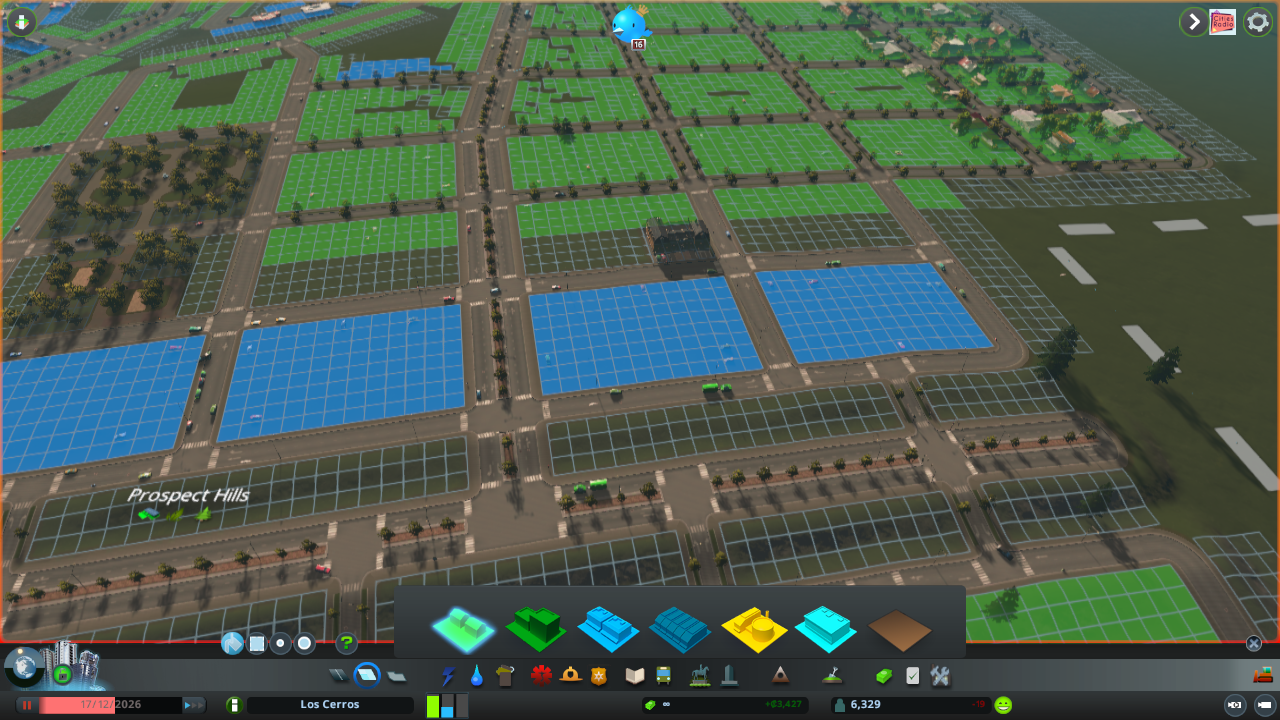
\includegraphics[width=\textwidth]{images/zoneo}
	\caption{Ejemplo de definición de zonas. En la azul las zonas comerciales y en verde las residenciales.}
	\label{fig:zoneo}
\end{figure}

\begin{itemize}
	\item \textbf{Residencial}: Corresponde a las casas donde la gente vivirá.
	\item \textbf{Comercial}: Se refiere a las tiendas y otros servicios que venden los productos creados por la industria o que son exportados.
	\item \textbf{Industrial}: Las zonas industriales proveen trabajo a los ciudadanos y crean los productos de consumo para los edificios comerciales.
	\item \textbf{Oficinas}: Las zonas de oficina dan trabajo solo a ciudadanos con alto nivel de estudios. Además no producen ni contaminación, ni tráfico, ni productos de consumo.
	\item \textbf{Servicios}: En esta categoría entran los edificios que no se pueden crear mediante zonas, si no que se fijan su construcción. Pertenecen al gobierno y dan servicios a los ciudadanos, como parques, cuarteles de policía, estaciones de buses, etc.
\end{itemize}

En este proyecto nos centraremos en las zonas industriales. Son una de las zonas que aumentan el tráfico intensamente, por lo que su planificación debe ser rigurosa. Las zonas industriales se dividen en varios tipos dependiendo de los recursos naturales que puedan usar, que pueden ser renovables (suelo fértil) o no renovables (petroleo y minerales).

\begin{itemize}
	\item \textbf{Genérica}: No tiene una especialización, por lo que corresponde a edificios genéricos. Es una de las más contaminantes pero es la base de la cadena de suministro en \cities. Proveen de trabajos para personas de estudios bajos.
	\item \textbf{Granjas}: Necesitan de suelo fértil (que es renovable) para producir recursos sin producir contaminación. Solo da trabajo para ciudadanos con nivel de estudios bajo.
	\item \textbf{Bosques}: No contamina el suelo pero genera un nivel de ruido significante. Consume también más electricidad que la industria genérica. También da trabajo para gente con nivel de estudios bajo.
	\item \textbf{Petróquímica}: Usa el suelo que contiene petróleo (que no es renovable) para producir combustible. Genera ingresos por impuestos altos, así como altos niveles de polución y consumo alto de energía.
	\item \textbf{Minera}: Usa zonas con minerales (recurso no renovable) para producir carbón. Produce menos polución e ingresos que la petroquímica pero usa más energía que la industria genérica.
\end{itemize}

\begin{figure}[h]
	\centering
	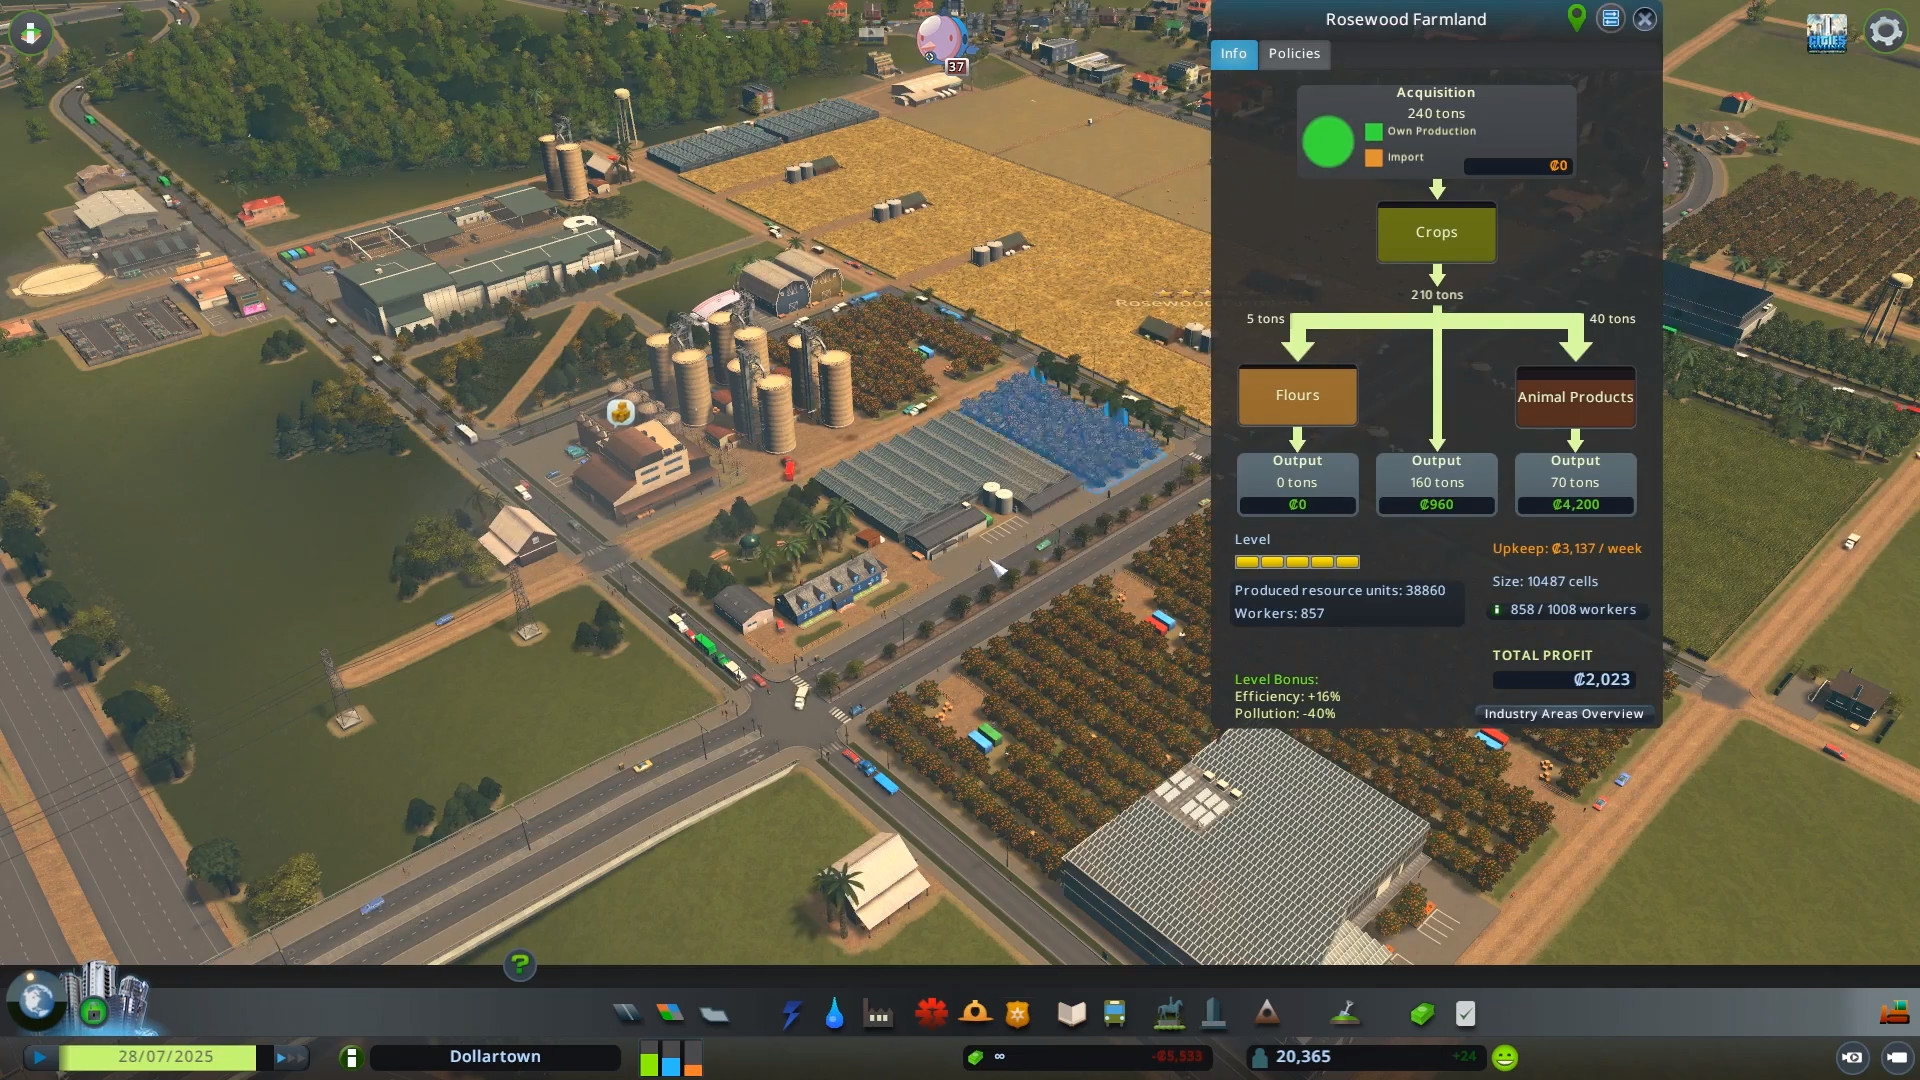
\includegraphics[width=\textwidth]{images/industries}
	\caption{Interfaz de gestión de recursos de la expansión \textit{Industries}}
	\label{fig:industry}
\end{figure}


Desde el lanzamiento de la expansión \textit{Industries}, se agregó un sistema producción, en donde se pueden procesar los recursos naturales hasta obtener productos de consumo de lujo. Para ello existen cinco tipos de edificios: extractores, procesadores, factorías, auxiliares y almacenes. Los edificios auxiliares dan zonas para que los trabajadores vivan y ofrecen mantenimiento, mientras que los almacenes sirven para guardar cada uno de los productos de cada una de las etapas.

Además, desde la expansión de \textit{Sunset Harbor} existe la industria pesquera, que agrega como recurso natural el pescado. Siguiendo el sistema de producción agregado en \textit{Industries}, este se puede procesar hasta obtener productos de consumo que se puedan exportar o vender en comercios. Dependiendo de la profundidad y el flujo del agua, se generará uno de los cuatro tipos de pescados: anchoas, atún, salmón y marisco. La polución en el agua provoca que desaparezcan este recurso del agua.

\section{Proceso de ingeniería}

En este capítulo se explica el proceso que se ha seguido para realizar el proyecto descrito. Se empezará explicando la metodología de desarrollo escogida y a continuación se expondrá y se desgranará la gestión de este trabajo.

\subsection{Metodología de desarrollo}
\label{subsec:metodologia}

A pesar de que en un primer se ha pensado que para la planificación de este proyecto se usaría la metodología de desarrollo SCRUM\cite{Schwaber:2001:ASD:559553}\cite{Schwaber:2004:APM:984028}, finalmente se ha optado por usar una amalgama entre distintas metodologías de desarrollo en espiral. Esto es debido a que SCRUM tiene unas características básicas que no se han tenido en cuenta a la hora de diseñar y desarrollar el proyecto, por lo que no sería correcto decir que se ha utilizado este tipo de metodología ágil:

\begin{itemize}
	\item \textbf{Flujo de trabajo}: El trabajo se divide en varias iteraciones entre una y cuatro semanas llamadas \textit{Sprint}, en donde en cada una de ellas se obtiene un incremento funcional del producto. Al comienzo de cada iteración se realiza una reunión en donde se identifican las tareas a realizar en esa iteración, realizando una estimación de todas; durante la realización de la iteración se realiza cada día una pequeña reunión en donde se comunica el estado actual; y, al finalizar una iteración se realiza una reunión que sirve como retrospectiva y alimentación para la próxima iteración.
	
	A la hora de realizar este proyecto, a pesar de que se ha dividido en varias iteraciones, realizando una reunión al principio de estos, y en cada iteración se finaliza con un producto funcional, el resto de elementos de la metodología SCRUM no se han llevado a cabo en la práctica.
	
	\item \textbf{Gestión de riesgos}: Uno de lo puntos de desarrollo con una metodología ágil es la de mantener una gestión de temprana de riesgos para evitar una gran desviación de la planificación. Esto se realiza mediante un panel que presenta listado ordenado de las tareas a realizar en el desarrollo total del proyecto, llamado \textit{Product backlog}. Estas tareas son las que estiman su duración y se incluyen en otro listado de tareas a realizar en cada iteración, llamado \textit{Sprint backlog}. Con esto se puede obtener una gráfica de evolución del proyecto llamado \textit{Burn down chart}, pudiendo detectar desviaciones y sobreasignaciones de forma visual debido a que también se marca el trabajo ideal de proyecto.
	
	Para este proyecto no se ha usado un desarrollo en Sprint porque no se ha realizado un seguimiento exhaustivo del mismo. En el caso de gestión de riesgos se ha usado el Product backlog como backlog de historias para hacer, sin hacer estimación.
\end{itemize}

Debido a todos estos factores expuestos, se podría indicar que la metodología usada finalmente está más cerca de una metodología basada en kanbanflow, en donde las tareas del product backlog se mueven a un tablero con columnas según el estado de la tarea; o una basada en modelos de prototipos, en donde se tiene en cuenta que cada prototipo resultante de una iteración es un modelo funcional del mismo, y en donde es revisado en la reunión de la siguiente iteración sin estar presente el cliente final, si no que solo con el director del proyecto. También en esta reunión se definen las tareas a realizar para el desarrollo del proyecto de cara a la nueva iteración.

\subsection{Gestión del proyecto}
\label{subsec:gestion}

A continuación se describirá la planificación llevada a cabo para la realización del proyecto, así como el coste y los recursos necesarios para la construcción del mismo.

\subsubsection{Planificación}

Volviendo a lo comentado en la Sección \ref{subsec:metodologia}, para la planificación se ha usado una metodología más parecida a un kanbanflow o un modelo de prototipos, dividiendo en varias tareas incrementales que, una vez terminadas, dan nuevas funcionalidades al producto final. Debido a la naturaleza del proyecto, estas tareas se han dividido en 3 épicas:

\begin{enumerate}
	\item \textbf{Generador del polígono industrial}: Las tareas presentes tienen que dar como producto final de esta épica un mod funcional para \cities. Dentro de esta épica tenemos las siguientes historias de usuario:
	\begin{enumerate}[label={\arabic*.}]
		\item \textbf{Crear prototipo de complejo industrial}: El complejo debe tener dos carreteras que se unan en la mitad con un cruce y en cada uno de los cuatro espacios se debe situar una nave.
		\item \textbf{Generar rejilla simple}: Se seleccionará una sección del mapa y se creará un conjunto de carreteras que formen una cuadrícula.
		\item \textbf{Conectan ClingoSharp con IndustryLP}: Se incluirá el proyecto ClingoSharp como dependencia de IndustryLP y se procederá a hacer una generación sencilla.
		\item \textbf{Funcionalidades extra}: Se añadirán a la selección de la región operaciones de movimiento de la región, cambio de tamaño y rotación de la misma.
		\item \textbf{Añadir restricciones/preferencias}: Para cada parcela, el usuario podrá proponer un edificio o prohibir la generación del mismo.
		\item \textbf{Establecer plantillas}: Se incluirá una lista de las distintas topologías de carreteras que el usuario podrá seleccionar, y que se usarán en vez de la cuadrícula.
		\item \textbf{Construir polígono}: Una vez seleccionado la solución de Clingo, el sistema deberá construir objetos servibles dentro del entorno de \cities.
	\end{enumerate}

	\item \textbf{Interfaz C\# con Clingo}: El resultado de esta épica es crear un producto final que sea una librería que actúe como binding de Clingo para C\#, que será usado por el mod creado en \cities:
	\begin{enumerate}[label={\arabic*.}]
		\setcounter{enumii}{7}
		\item \textbf{Generar biblioteca dinámica}: Como Clingo está escrito en C/C++, la idea es que se pueda crear una biblioteca dinámica nativa (.dll en Microsoft Windows, .so en GNU/Linux) que se pueda usar para ClingoSharp.
		\item \textbf{Cargar programa lógico sencillo}: Se deberían crear los módulos básico para poder invocar Clingo desde un programa en C\# y permitir que cargue un programa lógico.
		\item \textbf{Conectan ClingoSharp con IndustryLP}: Se incluirá el proyecto ClingoSharp como dependencia de IndustryLP y se procederá a hacer una generación sencilla.
		\item \textbf{Completar módulo Control}: El objetivo es poder leer cada uno de los átomos resultantes de un modelo estable. Además poder incorporar llamadas de forma asíncrona a Clingo.
		\item \textbf{Implementar módulo de modelos estables}: El objetivo es poder leer cada uno de los átomos resultantes de un modelo estable. Además poder incorporar llamadas de forma asíncrona a Clingo.
		\item \textbf{Añadir tests unitarios}: Se definirán los tests básico para las funcionalidades principales de Clingo.
	\end{enumerate}

	\item \textbf{Documentación}: El objetivo de esta épica es la de crear las diferentes documentaciones necesarias del proyecto. Se divide en:
	\begin{enumerate}[label={\arabic*.}]
		\setcounter{enumii}{13}
		\item \textbf{Memoria del proyecto}: Crear este documento que tendrá toda la información del proyecto.
		\item \textbf{Documentación del IndustryLP}: Generará los diagramas y la documentación de código necesaria.
		\item \textbf{Documentación de ClingoSharp}: Se crearán los diagramas y documentación del código necesaria.
	\end{enumerate}
\end{enumerate}

Considerando las tareas descritas anteriormente, en la Tabla \ref{table:dedicacion} podemos ver la dedicación en horas llevada a cabo para cada proyecto. Debido a que no se ha realizado una estimación antes de la realización, no tenemos un dato previsto, si no que es directamente el valor final tangible.

\begin{table}[!h]
	\centering
	\begin{tabular}{ c c }
		\bfseries{Tarea} & \bfseries{Tiempo (h)} \\
		\hline
		01 & 30 \\
		02 & 6 \\
		03 & 30 \\
		04 & 30 \\
		05 & 40 \\
		06 & 45 \\
		07 & 15 \\
		08 & 6 \\
		09 & 15 \\
		10 & 30 \\
		11 & 30 \\
		12 & 15 \\
		13 & 15 \\
		14 & 40 \\
		15 & 8 \\
		16 & 8 \\
		\hline
		\bfseries{Total} & 363 \\
		\hline
	\end{tabular}
	\caption{Desglose de la dedicación a las historias de usuario.}
	\label{table:dedicacion}
\end{table}

\subsubsection{Coste y recursos}

Para calcular el coste de los recursos humanos que ha supuesto este proyecto, aparte de las 363 horas totales se ha añadido un 10\% a mayores que incluye las reuniones de seguimiento por parte del director del proyecto.\\ 

Eso suma 37 horas al proyecto, dando un total de 400 horas total. Teniendo esto en cuenta, y siguiendo la Guía Salarial del Sector TI en Galicia \cite{guia_galicia}, se han estimado los costes que se pueden ver en la Tabla \ref{table:costehumano}.

\begin{table}[!h]
	\centering
	\begin{tabular}{ c c c c }
		\bfseries{Recurso} & \bfseries{Tiempo (h)} & \bfseries{Coste (\euro/h)} & \bfseries{Total} \\
		\hline
		Doctor Investigador & 37 & 24,00 & 888,00 \\
		Analista Programador & 363 & 9,00 & 3267,00 \\
		\hline
		\bfseries{Total} & 400 & & 4155,00 \\
		\hline
	\end{tabular}
	\caption{Coste de los recursos humanos del proyecto.}\label{table:costehumano}
\end{table}

\begin{table}[!h]
	\centering
	\begin{tabularx}{\textwidth}{ l X X X X }
		\bfseries{Recurso} & \bfseries{Vida (mes)} & \bfseries{Uso (mes)} & \bfseries{Coste (\euro)} & \bfseries{Total (\euro)} \\
		\hline
		Portátil & 48 & 10 & 800,00 & 166,67 \\
		\cities & $\infty$ & 10 & 27,99 & 27,99 \\
		Clingo & $\infty$ & 10 & - & 0 \\
		.NET Framework & $\infty$ & 10 & - & 0 \\
		Visual Studio & $\infty$ & 10 & - & 0 \\
		Github & $\infty$ & 10 & - & 0 \\
		LaTeX & $\infty$ & 10 & - & 0 \\
		\hline
		\bfseries{Total} & & & & 194,66 \\
		\hline
	\end{tabularx}
	\caption{Coste de los recursos materiales del proyecto.}\label{table:costematerial}
\end{table}

Por otro lado, en la \ref{table:costematerial} se recoge la lista de recursos materiales y lógicos necesarios para el desarrollo de este proyecto. Para el caso de los recursos \textit{hardware} se ha tenido en cuenta el tiempo de uso para este proyecto con respecto a su vida útil, mientras para los recursos \textit{software}, se ha preferido por usar herramientas y bibliotecas de uso libre y gratuitas, de ahí que el coste no esté contado para el resultado final. \\

Con todo esto se puede concluir que el coste total del proyecto asciende hasta \EUR{4349,66} en total.

\section{Análisis del software}

Una vez definido el sistema y planificada su construcción, se ha realizado un análisis en donde se identifican los requisitos que debe cumplir el software una vez terminado el proyecto.

\subsection{Requisitos funcionales}
\label{subsec:funcrequirements}

Los requisitos funcionales son aquellas condiciones indispensables que estipulan las funcionalidades que debe proporcional el sistema. Para este proyecto se ha recogido los diferentes requisitos:

\begin{itemize}
	\item Generación de un poligono industrial que sea legible por el videojuego \cities.
	\item Permitir añadir restricciones sobre ciertas zonas del mapa.
	\item Poder mostrar los resultados de la generación dentro del videojuego.
\end{itemize}

\subsection{Requisitos no funcionales}

Los requisitos no funcionales, por su contra, son aquellas condiciones indispensables que debe cumplir el sistema a la hora de diseñar e implementar. Para este proyecto se han tenido en cuenta estos requisitos:

\begin{itemize}
	\item Eficiencia y eficacia: El generador debe responder en el menor tiempo posible arrojando una respuesta óptima.
	\item Escalabilidad: El generador debe trabajar con mapas de diferentes tamaños, por lo que el sistema debe poder soportar cualquier tamaño de entrada.
	\item Usabilidad: La interfaz gráfica debe ser lo más sencilla posible, evitando que el usuario tenga que realizar tareas tediosas a la hora de construir mapas.
\end{itemize}

\section{Diseño del sistema}

Una vez definidos los requisitos se ha procedido a realizar el diseño software del sistema en cuestión, empezando a concretar la arquitectura propuesta y luego desarrollando los casos de uso y diagramas de clases.

\subsection{Arquitectura software}
\label{subsec:arquitectura}

Este proyecto se ha dividido en dos tipos de arquitectura dada la naturaleza del problema. Esto es debido a que estamos implementando diferentes paradigmas, y cada una tiene su forma de diseñarse. \\

\begin{figure}[!h]
	\centering
	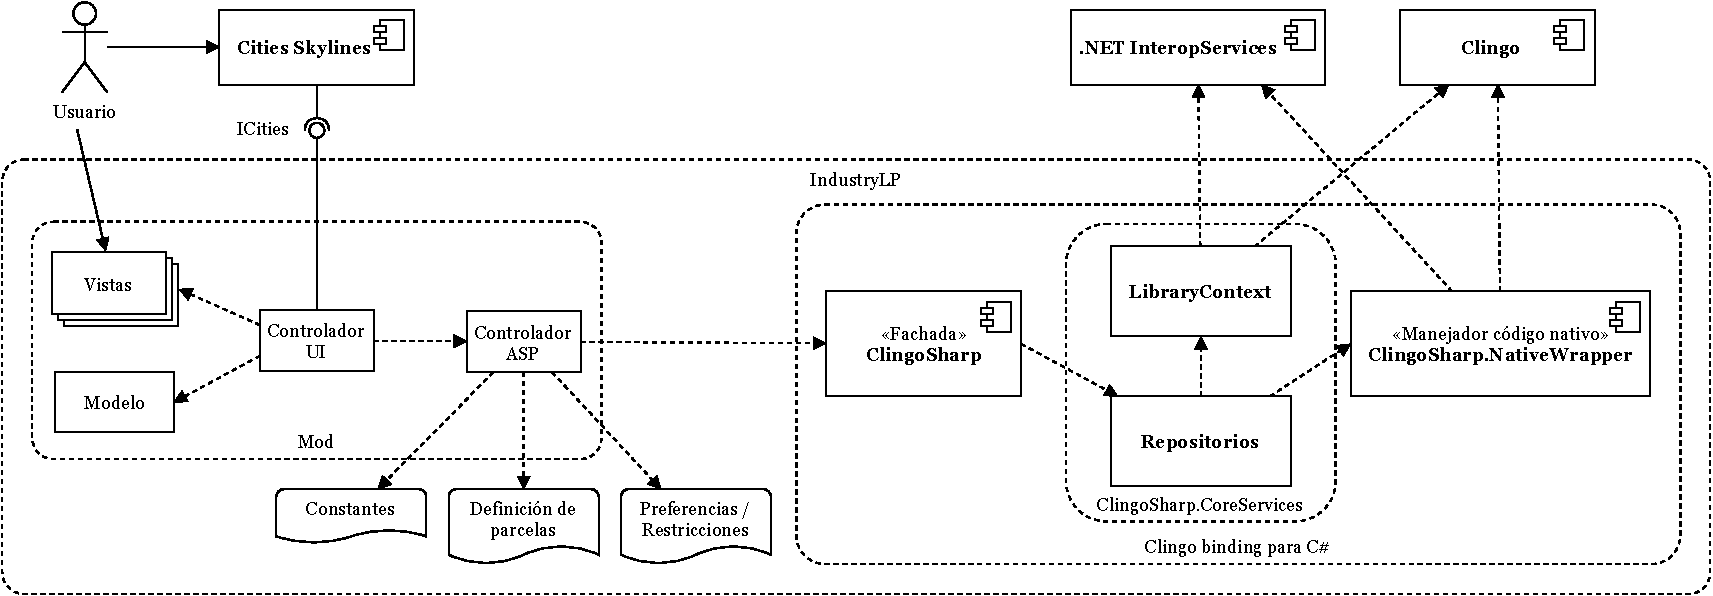
\includegraphics[width=\textwidth]{images/arquitectura-mod}
	\caption{Arquitectura del mod de \cities}
	\label{fig:arquitectura-mod}
\end{figure}

Como primera parte vamos a analizar la arquitectura del software que se ejecuta dentro de \cities. Tal y como se puede ver en la Figura \ref{fig:arquitectura-mod}, este se ha divido en dos capas para permitir sus reusabilidad en distintos proyectos. En la primera capa tendríamos la interfaz del mod en si mismo. Este se basa en una arquitectura Modelo-Vista-Controlador (MVC), en donde el controlador se encargará de reaccionar antes los eventos de las vistas, que son la parte que el usuario manipula, y modificar el modelo, que son los datos que se guardan en memoria en este caso. \\

Además, el controlador de la interfaz se conectará con el controlador del modulo ASP para hacer llamadas a Clingo y obtener el resultado de las preferencias, tal y como se explica en la Sección \ref{subsubsec:generator}. Este módulo a su vez llama a la segunda capa, que se corresponde con un \textit{binding} o adaptación de la API en C de Clingo para el lenguaje de programación C\#. Este binding usa como referencia final la API en Python de Clingo\footnote{https://potassco.org/clingo/python-api/5.4}, la cual está dividida en módulos. Es por eso que nos hemos basado en una arquitectura de repositorios, en donde hay una fachada que llama a cada una los distintos componentes, que contienen como contexto la referencia a la biblioteca de Clingo, y los cuales a su vez llaman a otro componente que se encarga de hacer la llamada a la API en C de Clingo. \\

\begin{figure}[!h]
	\centering
	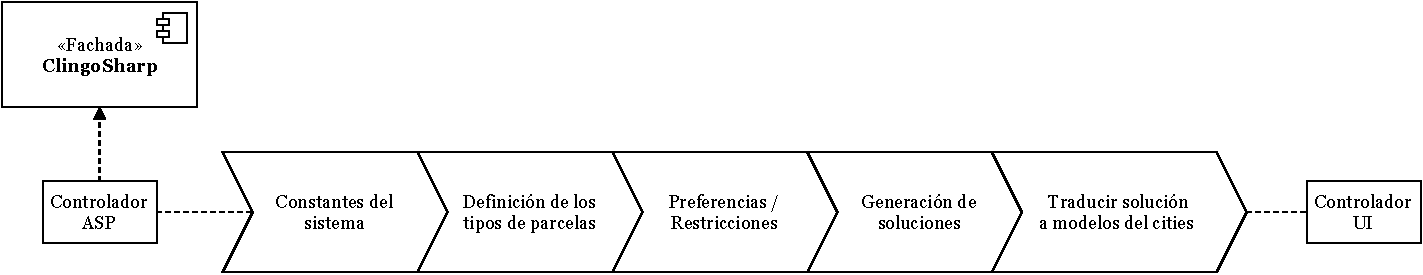
\includegraphics[width=\textwidth]{images/arquitectura-asp}
	\caption{Arquitectura del programa lógico}
	\label{fig:arquitectura-asp}
\end{figure}

En la segunda parte analizaremos la arquitectura del programa lógico. Como ya comentamos en la Sección \ref{subsec:asp}, para resolver un programa lógico necesitamos transformarlo a su equivalente con variables libres mediante un grounder, y obtener los modelos estables mediante un solver. Debido a que es un proceso de transformación se ha ideado el usar una arquitectura en \textit{pipeline}, en donde la salida de cada proceso es la entrada del siguiente. Tal y como se puede ver en la Figura \ref{fig:arquitectura-asp}, se ha divido en una etapa de definición de constantes del sistema lógico, una etapa de definición del los tipos de parcelas (obteniendo previamente la información de los modelos existentes en \cities), una etapa de preferencias o restricciones del tipo o posición de las parcelas, una etapa de obtención de los modelos estables, y una última etapa de traducción de cada átomo del modelo estable a un modelo que pueda comprender \cities. Cada una de las etapas se explicarán en la Sección \ref{subsubsec:generator}.

\subsection{Casos de uso}
\label{subsec:cases}

El sistema tiene en cuenta que se usará en todo momento por un único usuario, el cual llevará a cabo todas las funcionalidades propuestas en la Sección \ref{subsec:funcrequirements} a través de una interfaz gráfica. Estos requisistos funcionales se transforman, por tanto, en los casos de uso del sistema que se proponen en la Tabla \ref{table:casos-uso1}

\begin{figure}[!h]
	\centering
	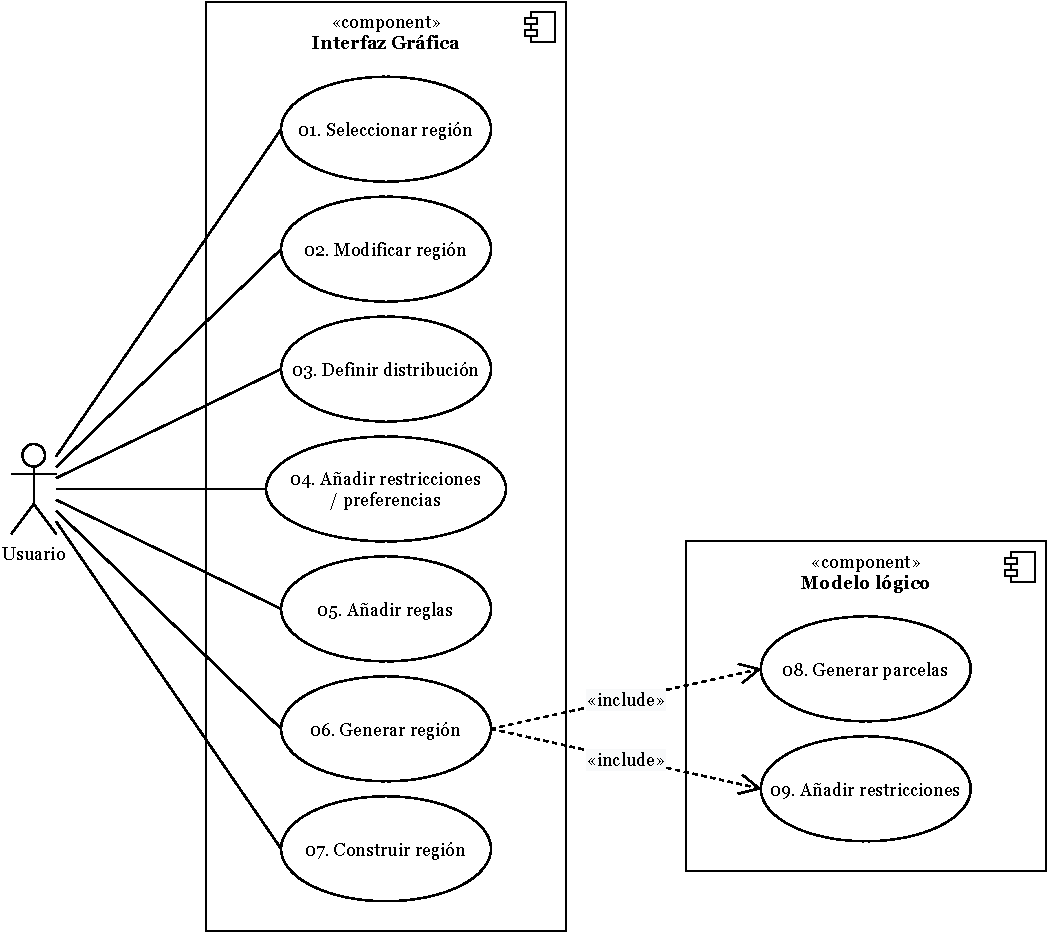
\includegraphics[width=\textwidth]{images/casos-uso}
	\caption{Diagrama de casos de uso del sistema propuesto}
	\label{fig:casos-uso}
\end{figure}

\begin{table}[!h]
	\begin{tabularx}{\textwidth}{ c c X }
		\bfseries{CU} & \bfseries{Nombre} & \bfseries{Descripción} \\
		\hline
		01 & Seleccionar región & El usuario puede pinchar en cualquier zona del mapa de \cities y marcar una región. \\
		\hline
		02 & Modificar región & Una vez marcada una región, el usuario puede cambiar el tamaño y la rotación de esta mediante movimiento del ratón. \\
		\hline
		03 & Definir distribución & Una vez establecida la región, el usuario puede indicar que tipo de topología de carreteras se va a generar en la región. \\
		\hline
	\end{tabularx}
	\caption{Descripción de casos de uso 1}
	\label{table:casos-uso1}
\end{table}

\begin{table}[!h]
	\begin{tabularx}{\textwidth}{ c c X }
		\bfseries{CU} & \bfseries{Nombre} & \bfseries{Descripción} \\
		\hline
		04 & \makecell{Añadir restricciones \\ / preferencias} & Dada una distribución, el usuario puede marcar que edificios prefiere generar y cuales quiere descartar de la generación. \\
		\hline
		05 & Añadir reglas & Antes de empezar a generar la región, el usuario puede modificar de forma opcional la generación indicando nuevas reglas escribiendolas en un campo de texto. \\
		\hline
		06 & Generar región & El sistema deberá generar una región válida y mostrarla. Para eso se apoyará de los casos de uso 08 y 09. \\
		\hline
		07 & Construir región & Una vez seleccionada la región que el usuario quiere construir, se invocará a \cities para que cree los objetos necesarios en el juego para que se pueda usar por la IA. \\
		\hline
		08 & Generar parcelas & El sistema deberá seleccionar un tipo edificio para cada tipo de parcela. \\
		\hline
		09 & Añadir restricciones & Una vez seleccionado el tipo de edificio, el sistema añadirá las restricciones de cada parcela para que el sistema lógico genere una solución que satisfaga dichas restricciones. \\
		\hline
	\end{tabularx}
	\caption{Descripción de casos de uso 2}
	\label{table:casos-uso2}
\end{table}

\subsection{Diseño del programa lógico}
\label{subsubsec:generator}

Retornando a lo comentado en la Sección \ref{subsec:arquitectura}, una de las piezas fundamentales de este proyecto es la definición de un generador de polígonos industriales en formato declarativo. Para ello usamos el paradigma de programación lógica, que usa la tecnología Answer Set Programming, tal y como se expone en la Sección \ref{subsec:asp}. \\

Con esto, el objetivo de este generador es intentar dar un modelo declarativo basado en reglas que corresponda en mayor o menor medida con la definición de un polígono industrial. A continuación explicamos el diseño de cada una de las etapas que consta el sistema de generación.

\subsubsection{Constantes del sistema lógico}

Como primer paso para la generación del polígono industrial, definimos unos átomos que nos servirán para indicar el tipo de algunas variables. En concreto hemos definido el átomo \texttt{row(X)}, que contiene la definición de cada fila, y \texttt{column(X)} que es la contraparte para columnas. En el caso de los tipos de edificio disponibles, se ha creado el átomo \texttt{str\_parcel(X)}, el cual guarda como string el nombre de cada uno de los edificios disponibles en \cities.

\subsubsection{Definición de los tipos de parcela}

Con las constantes ya definidas, se ha definido una regla para la generación de cada parcela \texttt{parcel(X, Y, B)} con una \textit{choice rule}. La \textit{choice rule} tiene cardinalidad 0 - 1, que se expresa como \textit{min \{p\} max} e indica que puede existir o no un átomo \texttt{parcel(X, Y, B)} dado un tipo de edificio \texttt{str\_parcel(B)} para cada celda \texttt{row(X), column(Y)}. \\

Con esto le decimos a Answer Set Programing que puede elegir cualquier combinación para cada parcela, incluyendo no generar una parcela de un tipo dato. Esto puede generar soluciones donde no existe parcelas, o donde para una parcela existen varias soluciones. Para restringir las soluciones a modelos estables en donde exista un solo átomo \texttt{parcel(X, Y, B)}, vamos a añadir un esquema de comprobación-restricción. Este esquema se basa en definir un átomo auxiliar que marque una comprobación concreta, y luego una restricción (una regla sin cabeza) para este átomo.

\newpage

\begin{lstlisting}[caption={Código para la generación de parcelas},captionpos=b,label=lst:parcel_def]
% Generacion %
0 { parcel(X, Y, B) : str_parcel(B) } 1 :- row(X), column(Y).

% Comprobacion %
sell_parcel(X, Y) :- row(X), column(Y), str_parcel(B), parcel(X, Y, B).

% Restriccion %
:- row(X), column(Y), not sell_parcel(X, Y).
:- parcel(X, Y, S1), parcel(X, Y, S2), str_parcel(S1), str_parcel(S2), row(X), column(Y), S1 != S2.
\end{lstlisting}

En nuestro caso usaremos como átomo auxiliar \texttt{sell\_parcel(X, Y)}, que nos indicará que existe una parcela en una posición, y como restricciones definiremos una regla para que no existan celdas sin el átomo \texttt{sell\_parcel(X, Y)}, y otra regla para que no existan celdas con tipos de edificio distintos.

\subsubsection{Preferencias/Restricciones de parcelas}

Con la definición de cada parcela a una posición dada hecha, añadiremos más reglas para delimitar la generación de los modelos estables a las preferencias del usuario. Para ello, desde la interfaz podemos indicar si queremos que un edificio se genere en una posición dada, o si queremos que un edificio no se genere nunca en una posición. \\

\begin{lstlisting}[caption={Preferencias de parcelas},captionpos=b,label=lst:preference_def]
% Preferencia de colocacion de parcelas
parcel(1, 1, "Cargoyard").
parcel(2, 3, "Wind turbine").
parcel(2, 2, "Cargoyard").
parcel(3, 1, "General Factory 3x2").
        ...

% Restricciones del tipo de edificio
:- parcel(4, 1, "General Factory 2x2").
:- parcel(1, 2, "Forestry 4x4").
:- parcel(2, 2, "Forestry 4x3").
\end{lstlisting}

En la primera parte vamos a traducir las preferencias a hecho, que son los propio átomo, o también se pueden ver como reglas sin cola y actúan como valores de verdad dentro del modelo lógico. En el segundo caso, se traducirán a restricciones o reglas sin cabeza, tal y como vimos en la sección anterior. En el Listado \ref{lst:preference_def} vemos ejemplos de estas preferencias. \\

Uno de los resultados lógicos que podemos tener aquí es que el usuario ponga tanto como preferencia como restricción el mismo tipo de edificio. Aquí el resultado que nos devuelve clingo es que el modelo es insatisfactible, es decir, no existe ningún modelo estable que cumpla con el programa lógico, tal y como se muestra en la Figura \ref{fig:clingo-unsat}. \\

\begin{figure}[!h]
	\centering
	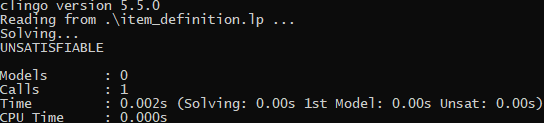
\includegraphics[width=\textwidth]{images/clingo-unsat}
	\caption{Ejemplo de un programa lógico sin solución}
	\label{fig:clingo-unsat}
\end{figure}

Otras formas de delimitar la generación es mediante las distancias y la topología de la generación. Esto nos permite hacer reglas más complejas en donde indiquemos restricciones más avanzadas, como que no queremos que dos tipos de edificios estén cerca, por ejemplo en el caso de que sea industria contaminante con industria verde. Para ello podemos usar algún algoritmo, como distancia de manhattan (tal y como se muestra en el Listado \ref{lst:manhattan_def}) o k-vecino más cercano. \\

\newpage

\begin{lstlisting}[caption={Cálculo de la distancia del taxista en Aswer Set Programing},captionpos=b,label=lst:manhattan_def]
distance(S1, S2, |X1-X2|+|Y1-Y2|) :- parcel(X1, Y1, S1), parcel(X2, Y2, S2), X1 != X2, Y1 != Y2.
neighbour(S1, S2) :- distance(S1, S2, 1).
\end{lstlisting}

Para delimitar la generación con este tipo de reglas, podemos usar los átomo que acabamos de crear como una estrategia de \textit{divide y vencerás}, introduciendo estos átomos en hechos o en prohibiciones. Esto se ve reflejado en el Listado

\begin{lstlisting}[caption={Prohibiciones de generación de edificios},captionpos=b,label=lst:distance_rules]
neighbour("Forestry 3x3", "Forestry 3x2").
neighbour("Forestry 3x4", "Forestry 3x2").
neighbour("Forestry 3x3", "Forestry 3x2").

:- distance("Forestry 3x3", "Farm Village", D), D < 4.
:- distance("Forestry 3x4", "Farm Village", D), D < 4.
\end{lstlisting}

\subsection{Implementación}
\label{subsec:implementacion}

Una vez analizado el proyecto en cuestión, y explicado como funciona el programa lógico, pasaremos a detallar el diseño de los componentes principales de los sistemas creados para usar en \cities. \\

Primeramente empezaremos explicando como funcionan las diferentes acciones en \industrylp. Pensando en su reusabilidad, y que en un futuro el número de acciones pueda crecer, se ha pensado en implementarlas usando un patrón estrategia. Tal y como se muestra en la Figura \ref{fig:actions}, cada acción deriva de la clase \texttt{ToolAction}.\\

\begin{figure}[!h]
	\centering
	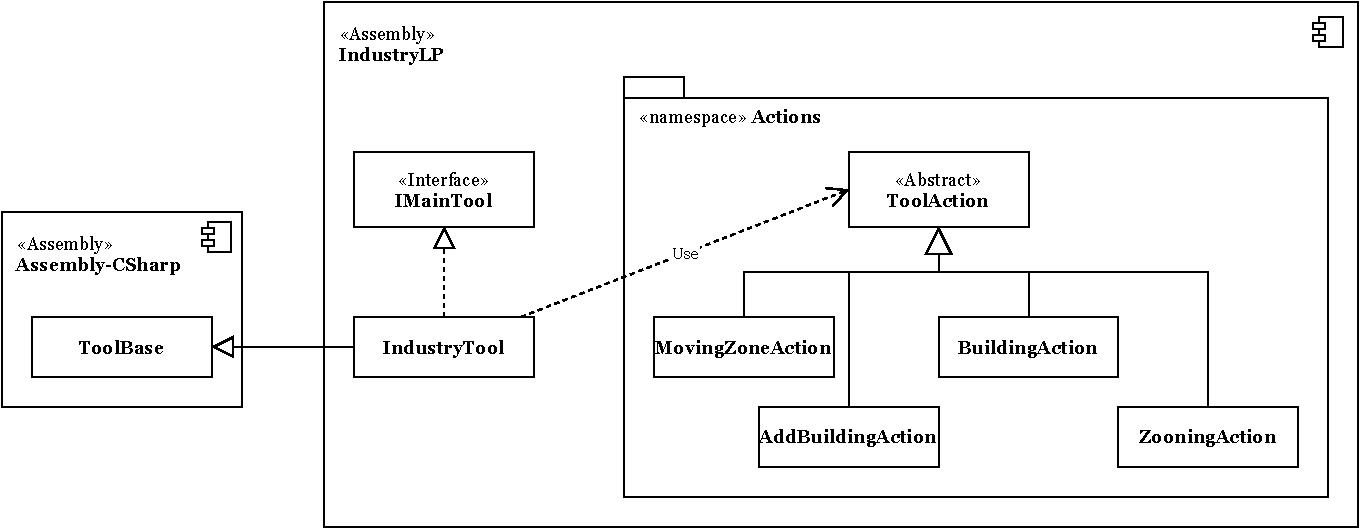
\includegraphics[width=\textwidth]{images/actions}
	\caption{Acciones de la interfaz}
	\label{fig:actions}
\end{figure}

Esta clase abstracta define una serie de métodos comunes que corresponden al ciclo de vida pensado para cada una de las acciones, representados en la Figura \ref{fig:action-lifecycle}. El ciclo de vida de una accion es controlado por la clase \texttt{IndustryTool}, que a su vez deriva de \texttt{ToolBase}, una clase abstracta que nos proporciona la interfaz de \cities y que también tiene un ciclo de vida, pero que es controlado por el propio juego.

\begin{figure}[!h]
	\centering
	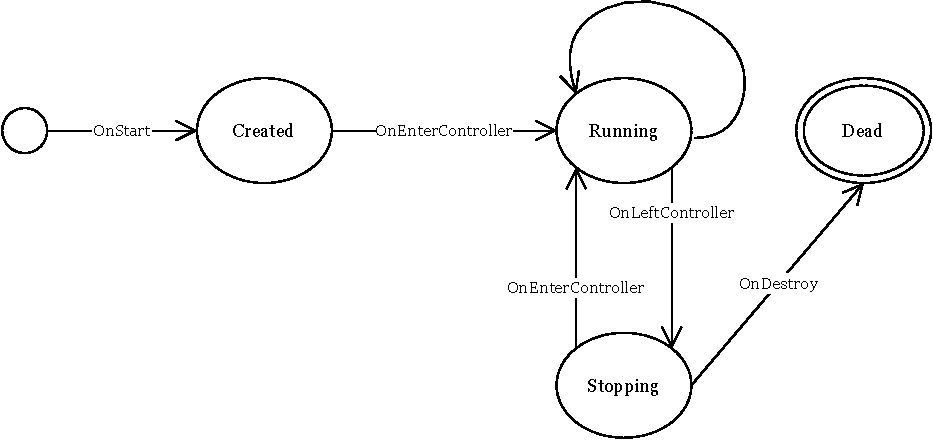
\includegraphics[width=\textwidth]{images/action-lifecycle}
	\caption{Ciclo de vida de una actividad}
	\label{fig:action-lifecycle}
\end{figure}

Es por eso que, dependiendo del estado en el que se encuentre el juego y la interfaz, la clase \texttt{IndustryTool} delegará en cada una de las acciones. Además, \texttt{IndustryTool} implementa la interfaz \texttt{IMainTool}, que define una serie de métodos que pueden usan las acciones para cambiar de estado o ejecutar otra acción, evitando así el acoplamiento entre \texttt{IndustryTool} y cada una de las acciones concretas. \\

\newpage

Con respecto a la generación de distribuciones, pensando también en la reusabilidad y en la implementación de nuevas topologías de parques industriales en un futuro, también se optó por usar un patrón de diseño, en este caso de \textit{Template Method}. El diseño de la generación de distribuciones se muestra en la Figura \ref{fig:distributions}.

\begin{figure}[!h]
	\centering
	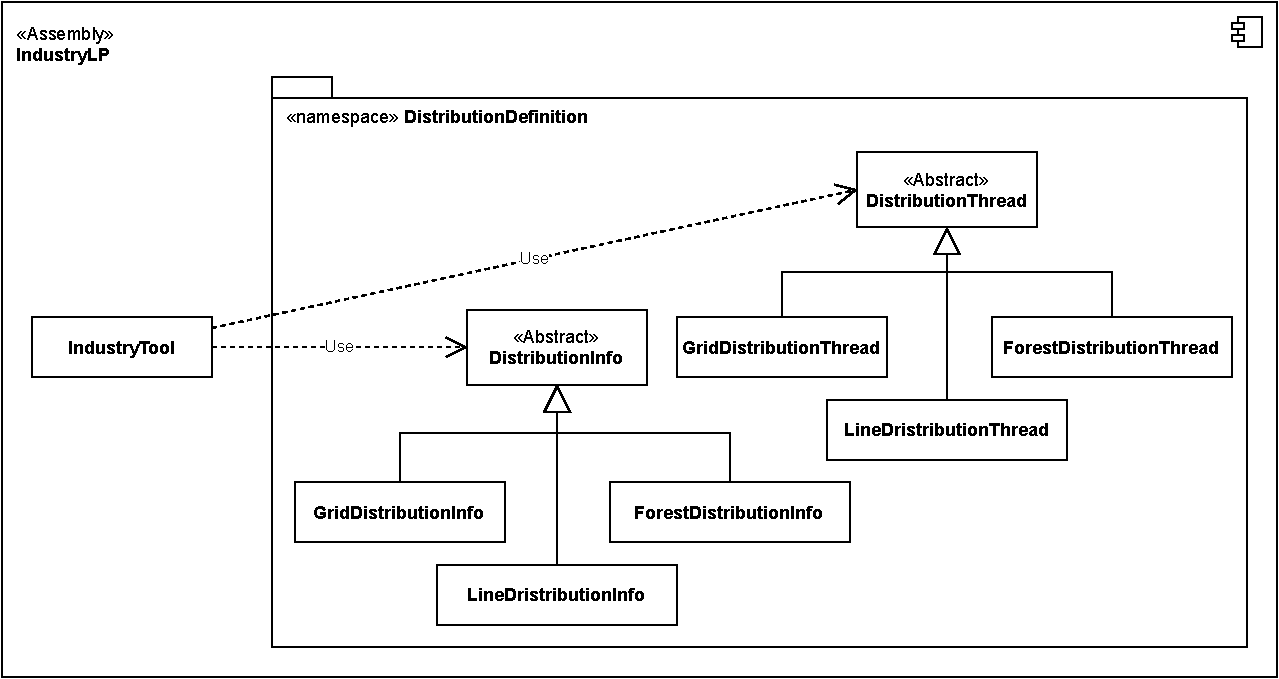
\includegraphics[width=\textwidth]{images/distribuciones}
	\caption{Definición de las distribuciones}
	\label{fig:distributions}
\end{figure}

Aquí, existen dos clases abstractas: \texttt{DistributionThread}, que define los métodos para la ejecución del algoritmo de generación de la distribución, el cual a diferencia del problema principal, este está implementado de forma imperativa; y \texttt{DistributionInfo}, que contiene la información resultante de la generación del algoritmo, y que define métodos de navegación de parcelas según la distribución. \\

En el caso del sistema que se encarga de conectar y ejecutar la biblioteca de Clingo, se ha optado por una arquitectura de tipo repositorio, tal y como se muestra en la Figura \ref{fig:clingosharp-repository}. Cada módulo de Clingo conecta con un módulo del componente \textit{ClingoSharp.NativeWrapper}, que se encargar de enlazar dinámicamente las funciones de la API en C con métodos internos de cada módulo. Estos módulos a su vez exponen funciones con tipos de datos manejados por C\# mediante interfaces, que derivan de una interfaz general llamada \texttt{IClingoModule}. \\

\begin{figure}[!h]
	\centering
	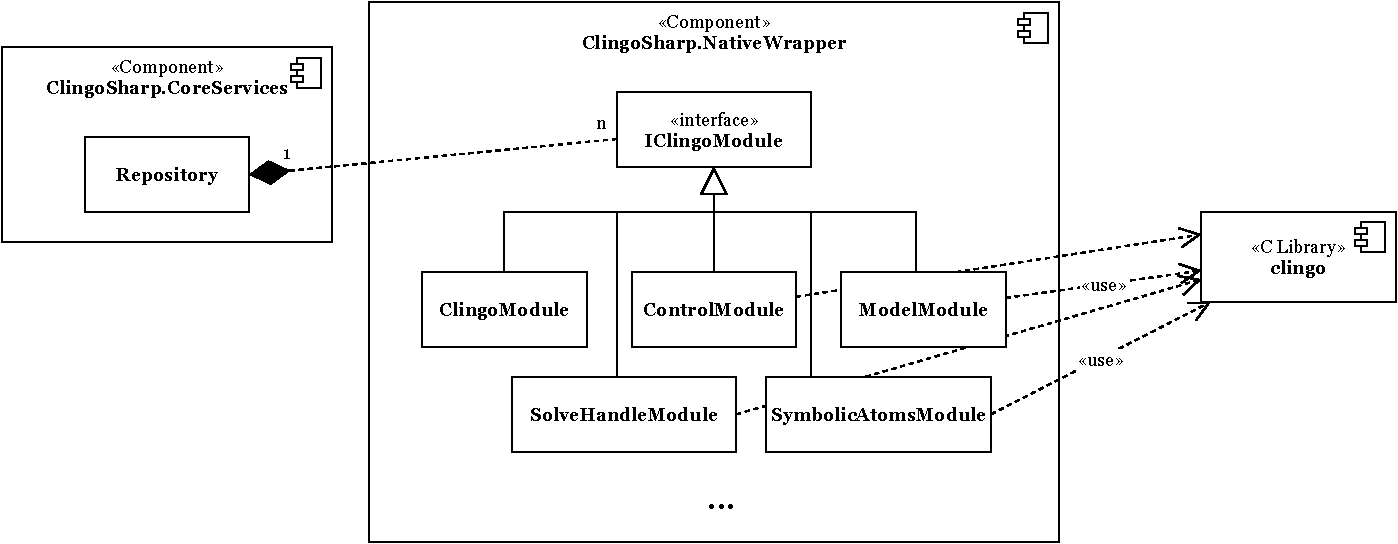
\includegraphics[width=\textwidth]{images/repository}
	\caption{Arquitectura de ClingoSharp}
	\label{fig:clingosharp-repository}
\end{figure}

En el caso del componente \texttt{ClingoSharp.CoreService}, este implementa la clase \texttt{Repository}, que contiene una composición de cada uno de los módulos. Esto es debido a que antes se pasa a memoria la biblioteca en Clingo, haciendo uso de los servicios disponibles en cada sistema operativo y de .NET Framework. Una vez realizada la carga en memoria, se procede a cargar dinamicamente cada uno de los módulos marcados con la interfaz \texttt{IClingoModule} del componente \textit{ClingoSharp.NativeWrapper}, y que finalmente son expuestos por nuestro repositorio. \\

En la Figura \ref{fig:clingosharp} se muestran las dependencias de cada uno de los distintos módulos. A pesar de lo complicado que parece, la arquitectura en repositorio nos permite abstraer la parte de enlazado de nuestro programa con la biblioteca nativa de Clingo, del enlazado de cada uno de los diferentes punto de control de la biblioteca, además de exponer una API limpia de Clingo en C\#. Otro punto a favor de esta arquitectura es que también actúa como wrapper, permitiendo cambiar entre distintas versiones de la biblioteca nativa de Clingo sin cambiar nuestro código, así como de implementar otra biblioteca de Aswer Set Programming en C\#. \\

\begin{figure}[!h]
	\centering
	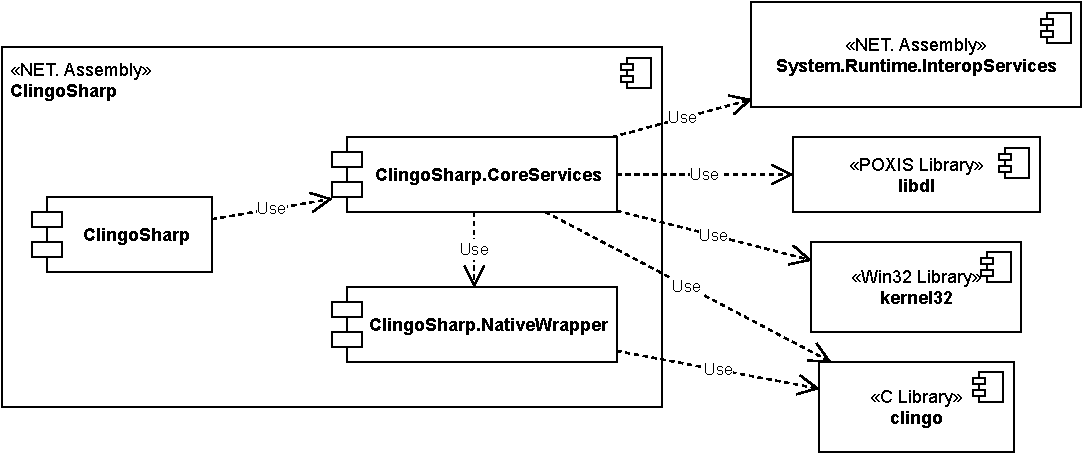
\includegraphics[width=\textwidth]{images/clingosharp}
	\caption{Dependencias de ClingoSharp}
	\label{fig:clingosharp}
\end{figure}

Para finalizar, cabe destacar que cada una de las capas (IndustryLP y ClingoSharp) se ejecuta en paralelo, pudiendo el primero enviar mensajes a ClingoSharp sin causar que la interfaz se congele, ademas de servir como recolector de errores que se puedan originar en nuestro programa lógico sin afectar a \cities.